\documentclass[a4papert,12pt]{report}% autres choix : book, report
\usepackage{lmodern}
\usepackage[utf8]{inputenc}
\usepackage{amsmath}
\parindent=1cm
%\parindent=15pt
\usepackage{amssymb}
\usepackage{amsthm}
\usepackage{mathrsfs}
\usepackage[francais,english]{babel}
\usepackage[T1]{fontenc}
\usepackage{float}
\usepackage{eurosym}  
\usepackage{array}
\usepackage{multirow}
\usepackage{wrapfig}
\usepackage{graphicx}
\usepackage{hyperref}
\usepackage{pythontex} 
\usepackage{listings}
\usepackage{xcolor}
\definecolor{codegreen}{rgb}{0,0.6,0}
\definecolor{codegray}{rgb}{0.5,0.5,0.5}
\definecolor{codepurple}{rgb}{0.58,0,0.82}
\definecolor{backcolour}{rgb}{0.95,0.95,0.92}
\lstdefinestyle{mystyle}{
    backgroundcolor=\color{backcolour},   
    commentstyle=\color{codegreen},
    keywordstyle=\color{magenta},
    numberstyle=\tiny\color{codegray},
    stringstyle=\color{codepurple},
    basicstyle=\ttfamily\footnotesize,
    breakatwhitespace=false,         
    breaklines=true,                 
    captionpos=b,                    
    keepspaces=true,                 
    numbers=left,                    
    numbersep=5pt,                  
    showspaces=false,                
    showstringspaces=false,
    showtabs=false,                  
    tabsize=2
}
\lstset{style=mystyle}
\hypersetup{
    colorlinks=true,
    linkcolor=blue,
    filecolor=magenta,      
    urlcolor=cyan,
    pdftitle={Overleaf Example},
    pdfpagemode=FullScreen,
    }
\usepackage{textcomp}
\usepackage{layout}
\renewcommand{\emph}{\texttt}
\usepackage{url}
\usepackage{color}
%\usepackage{pdfpages}
%\includepdf[pages=3-5]{document}
\usepackage{setspace}
%\usepackage[url color=black, % Liens vers une page web
%link color=black, % Liens internes au document
%color links=true]{hyperref}%color ma table de matière en bleue
%\usepackage[top=3 cm, bottom=2cm, left=3cm, right=3cm]{geometry}
\usepackage[top=1 cm, bottom=2cm, left=2cm, right=2cm]{geometry}
%\usepackage[top=1 cm, bottom=1cm, left=1.5cm, right=1.5cm]{geometry}
\setcounter{tocdepth}{2}
\onehalfspacing
%\fontfamily{pnc}\selectfont.
\usepackage{graphicx}
\usepackage{subcaption}

\begin{document}

\chapter*{\normalsize{\textbf{CERTIFICATE}}}
%\addstarredchapter{CERTIFICATE}
\addcontentsline{toc}{section}{\normalsize{\textbf{CERTIFICATE}}}
\paragraph{}
This is to certified that the project report title "\textbf{Meteorological satellite :  sensing principles, data collection and analysis}" is work done by Mr.YOUNKAP NINA Duplex,  Air Traffic Controller - MEng Degree in Computer Science, IMD Advance Training in Meteorological Instrumentation \& Information System Batch No. IX, ICITC. Under my supervision.
\paragraph{}
I recommend the project report for submission.
\vspace{10\baselineskip}
\begin{flushleft}
	\begin{tabular}{ll} 
	\textbf{Place }:			Garoua &  \\
	\vspace{ 3\baselineskip}
	\textbf{Date } :			07/03/2021 & \\
	\end{tabular}
\end{flushleft}


\newpage

\chapter*{\normalsize{\textbf{ACKNOWLEDGEMENT}}}
%\addstarredchapter{ACKNOWLEDGEMENT}
\addcontentsline{toc}{section}{\normalsize{\textbf{ACKNOWLEDGEMENT}}}
\paragraph{}
I am grateful to Mr. TCHAMABO Urbain, Forecaster - MEng Degree in Meteorology, who has guided me on this project with his immense knowledge and experience. 
\paragraph{}
I am grateful to officers and staffs of training section for the support extended throughout the training period.
\paragraph{}
I am grateful to Ms AFANE Bélinda Cyrielle, Local Coordinator - MEng Degree in Airport Management for her support.



\newpage

%\tableofcontents
%\addcontentsline{toc}{section}{\normalsize{\textbf{TABLES DES MATIÈRES}}}

%\input{sigle.tex}
\newpage


%\selectlanguage{francais}% on s'assure que la langue est bien le français

%\input{resume.tex}



\selectlanguage{english}% on change de langue pour le résumé en anglais


%\input{abstract.tex}



%\selectlanguage{francais}% on revient à la langue d'origine
%\listoftables
%\addcontentsline{toc}{section}{\normalsize{\textbf{LISTE DES TABLEAUX}}}

%\listoffigures
%\addcontentsline{toc}{section}{\normalsize{\textbf{LISTE DES FIGURES ET ILLUSTRATIONS}}}



%\input{annexe.tex}
%\newpage
%\setcounter{page}{1}
%\pagenumbering{arabic}

%\input{introduction1.tex}
\chapter*{\normalsize{\textbf{INTRODUCTION}}}
%\addstarredchapter{INTRODUCTION}
\addcontentsline{toc}{section}{\normalsize{\textbf{INTRODUCTION}}}
\paragraph{}
The general concept behind remote sensing is to monitor Geographical, Biological and Physical characteristics of Land, Water and Atmosphere.
It can offer a snap shot of state of the system at a particular point in time and 2D space.
A combination of such “observations” gives valuable Information on the resource under study.
These Information flow from analysts to managers to decision makers for successful interventions. 
In this report our focus is remote sensing for weather observation 
\setcounter{page}{1}
\pagenumbering{arabic}
\newpage
  
%\chapter{\normalsize{BACKGROUND OF SATELLITE REMOTE SENSING}}
\chapter{\normalsize{BASIC PRINCIPLES OF SATELLITE REMOTE SENSING}}
\section{Definition}
\paragraph{}
\textbf{Remote sensing} is the science (and to some extent, art) of acquiring information about the Earth's surface without actually being in contact with it. This is done by sensing and recording reflected or emitted energy and processing, analysing, and applying that information.
\paragraph{}
In much of remote sensing, the process involves an interaction between incident radiation 
and the targets of interest. This is exemplified by the use of imaging systems where the 
following seven steps are involved. However that remote sensing also involves the 
sensing of emitted energy and the use of non-imaging sensors. 
\end{description}
\begin{figure}[H]
\begin{center}
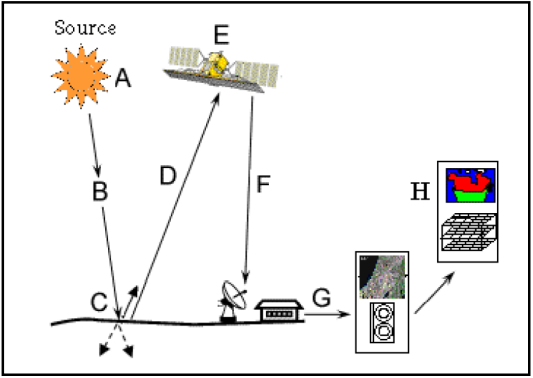
\includegraphics[scale=0.8]{image0.png} %\cite{umhe}
\end{center}
\caption{Remote sensing process}
\label{Remote sensing process}%\cite{ABIA}
\end{figure}
\begin{description}
\item[Step 1-Energy Source or Illumination (A)] : the first requirement for remote sensing is to have  an energy source which illuminates or  provides electromagnetic energy to the target of interest.
\item[Step 2-bandRadiation and the Atmosphere (B) band]: as the energy travels from its source to the target, it will come in contact with and interact with the atmosphere it passes through. This interaction may take place a second time as  the energy travels from the target to the sensor. 
\item[Step 3-Interaction with the Target (C)] : once the energy makes its way to the target through the atmosphere, it interacts with the target depending on the properties of both the target and the radiation.
\item[Step 4-Recording of Energy by the Sensor (D)] : after the energy has been scattered by, or emitted from the target, we require a sensor (remote - not in contact with the target) to collect and record the electromagnetic radiation. 
\item[Step 5-Transmission, Reception, and Processing (E)]: the energy recorded by the sensor has to be transmitted, often in electronic form, to a receiving and processing station where the data are processed into an image (hardcopy and/or digital).
\item[Step 6-Interpretation and Analysis (F)] the processed image is interpreted, visually and/or  digitally or electronically, to extract information about the target which was illuminated. 
\item[Step 7-Application (G) ] the final element of the remote sensing process is achieved when we  apply the information we have been able to extract from the imagery about the target in order  to better understand it, reveal some new information, or assist in solving a particular problem. 

%\section{Présentation du lieu du stage}
\section{Electromagnetic Spectrum}
\paragraph{}
Solar radiation can be divided into different wavelengths call EM spectrum:
\begin{enumerate}
\item Ultra violet (UV) [3-400 nm] 
\item Visible (Vis) [0.4-0.7 µm]
\item Infrared Red (IR) [0.7-100 µm]
\begin{enumerate}
\item Reflected IR [0.7-3 µm]
\begin{itemize} 
\item Near IR [0.7-1.5 µm]
\item Shortwave IR [1.5-3 µm]
\end{itemize}
\item Emitted IR or TIR [3-100 µm] 
\begin{itemize} 
\item Midwave IR [3-8 µm]
\item Longwave IR [8-15 µm]
\item Far IR [15-100 µm]
\end{itemize}
\end{enumerate} 
\item Microwave (MW) [1 mm – 1m]
\begin{description}
\item[P band]: 0.3 - 1 GHz (30 - 100 cm)
\item[L band]: 1 - 2 GHz (15 - 30 cm)
\item[S band]: 2 - 4 GHz (7.5 - 15 cm)
\item[C band]: 4 - 8 GHz (3.8 - 7.5 cm)
\item[X band]: 8 - 12.5 GHz (2.4 - 3.8 cm)
\item[Ku band]: 12.5 - 18 GHz (1.7 - 2.4 cm)
\item[K band]: 18 - 26.5 GHz (1.1 - 1.7 cm)
\item[Ka band]: 26.5 - 40 GHz (0.75 - 1.1 cm)
\end{description}
\end{enumerate}
\begin{figure}[H]
\begin{center}
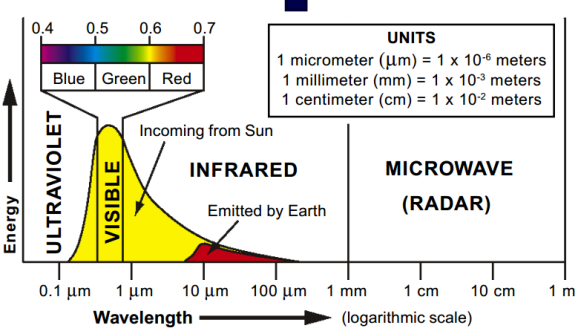
\includegraphics[scale=0.8]{image1.png} %\cite{umhe}
\end{center}
\caption{Electromagnetic spectrum}
\label{Electromagnetic spectrum}%\cite{ABIA}
\end{figure}
Most Multispectral satellite can acquire data in visible and infrared region (including the thermal infrared region).  Now days there is an increasing demand for data in microwaves region, because the microwave energy can penetrate through the cloud.
\section{Source of radiation}
\paragraph{}
We have two majors source of radiation: Sun and Earth.
\begin{description}
\item[Sun] is the mayor source of radiation with highest energy in visible, near infrared and short-wave infrared region as shown on picture above.
\item[Earth surface] can also emit energy usually in thermal Infrared and microwaves region.
\end{description}
\begin{figure}[H]
\begin{center}
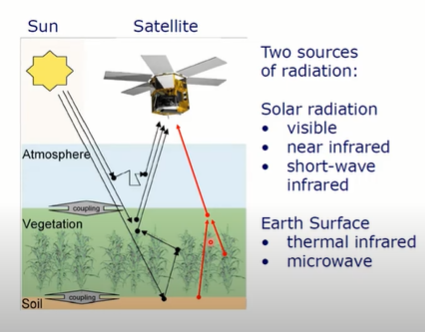
\includegraphics[scale=0.8]{images2.png} %\cite{umhe}
\end{center}
\caption{Source of radiation}
\label{Source of radiation}%\cite{ABIA}
\end{figure}
\section{Interaction in the atmosphere}
\paragraph{}
Before radiation used for remote sensing reaches the Earth's surface it has to travel through some distance of the Earth's atmosphere. Different processes happening due to the presence of particles and gases in the atmosphere. Some get \textbf{scattered}, some get \textbf{absorbed}, some managed to transmit through the atmosphere and get \textbf{absorbed}  by the earth, and some get \textbf{reflected} . This reflected energy is capture by the sensor on board of satellite. They are some energies emitted from the earth which are directly proportional to the heat of that particular object. This emitted energy can also be recorded by sensor on board of satellite if that sensor has capabilities to record energy in thermal infrared region. A sensor on board a satellite can record \textbf{remitted}  or \textbf{reflected} radiation depending on the capabilities of the sensors.
\begin{figure}[H]
\begin{center}
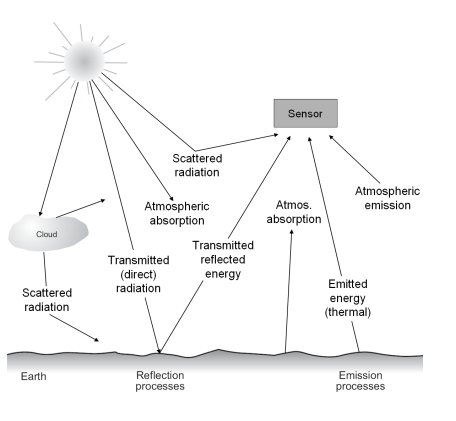
\includegraphics[scale=0.8]{image3.png} %\cite{umhe}
\end{center}
\caption{radiance at the sensor}
\label{radiance at the sensor}%\cite{ABIA}
\end{figure}
\section{How does it work ?}
As we said above, the energy is either emitted or reflected. And this emission or reflection on energy depend on he targets of interest e.g. cloud, trees, water, etc. They all have different level of reflectance, and this radiation of energy from different targets type will be recorded by the sensor installed in the satellite. Many time what is record by satellite is directly proportional to top of the atmosphere (TOA) "level at which the effect of absorption and scattering is not relevant". The energy recorded at sensor is proportional to what could be at the top of atmosphere e.g. temperature and humidity recorded is equal to brightness temperature (TOA Temperature), and we have to apply some correction convert brightness temperature to surface temperature. The same go to reflectance, we have to convert TOA radiance energy to surface reflectance energy. This process is call atmospheric correction. This how satellite records energy and how it correspond to different targets of interest.
\begin{figure}[H]
\begin{center}
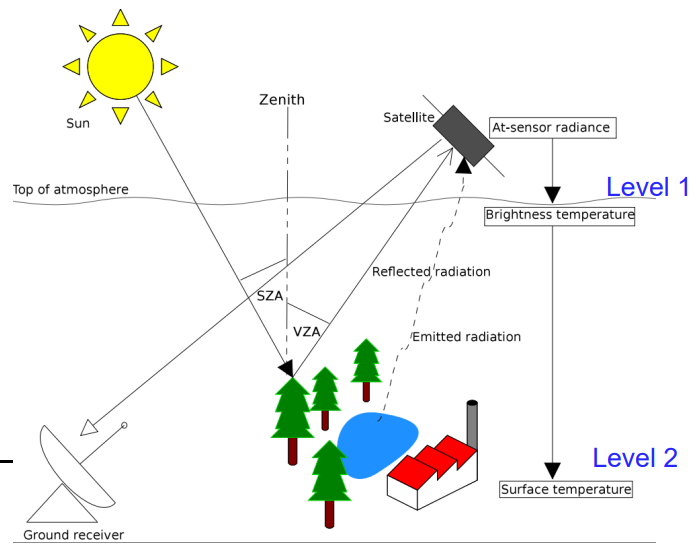
\includegraphics[scale=0.8]{image4.png} %\cite{umhe}
\end{center}
\caption{Sattelite remote seinsing}
\label{Sattelite remote seinsing}%\cite{ABIA}
\end{figure}
\section{Category of satellite}
There are different category of satellite based on:
\begin{description}
\item[Source of energy]: passive and active Sensors.
\item[Orbit]: polar, geo-stationary and sun-synchronous.
\item[Resolutions]: spatial, spectral, radiometric and temporal.
\item[Objectives]: communication, weather, navigation, earth observation, etc.
\end{description}













   
\newpage

%\chapter{\normalsize{BACKGROUND OF SATELLITE REMOTE SENSING}}
\chapter{\normalsize{CASE STUDY: GOES-R Series}}
\section{GOES project current status}
\paragraph{}
The Geostationary Operational Environmental Satellite Program (GOES) is a joint effort of  National Aeronautics and Space Administration (NASA) and the National Oceanic and Atmospheric Administration (NOAA). The GOES system currently consists of GOES-13, operating as GOES-East, in the eastern part of the constellation at 75 degrees west longitude and GOES-15, operating as GOES-West, at 135 degrees west longitude. The GOES-R series will maintain the two-satellite system implemented by the current GOES series. However, the locations of the operational GOES-R satellites will be 75 degrees west longitude and 137 degrees west longitude. The latter is a shift in order to eliminate conflicts with other satellite systems. The GOES-R series operational lifetime extends through December 2036.
These spacecraft help meteorologists observe and predict local weather events, including thunderstorms, tornadoes, fog, hurricanes, flash floods and other severe weather. In addition, GOES observations have proven helpful in monitoring dust storms, volcanic eruptions and forest fires.The benefits that directly enhance the quality of human life and protection of Earth's environment include:
\begin{itemize} 
\item Supporting the search-and-rescue satellite aided system (SARSAT).
\item Contributing to the development of worldwide environmental warning services and enhancements of basic environmental services.
\item Improving the capability for forecasting and providing real-time warning of solar disturbances.
\item Providing data that may be used to extend knowledge and understanding of the atmosphere and its processes.
\end{itemize}	
The next series of GOES satellites includes GOES-R, S, T and U.
\begin{figure}[H]
\begin{center}
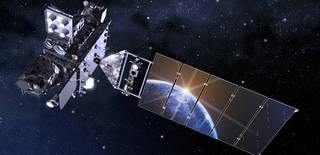
\includegraphics[scale=0.8]{goes-r_main_earth_reflection_panel_image.jpg} %\cite{umhe}
\end{center}
\caption{Goes-R Series}
\label{Goes-R Series}%\cite{ABIA}
\end{figure}
\section{GOES Project History}
\begin{figure}[H]
\begin{center}
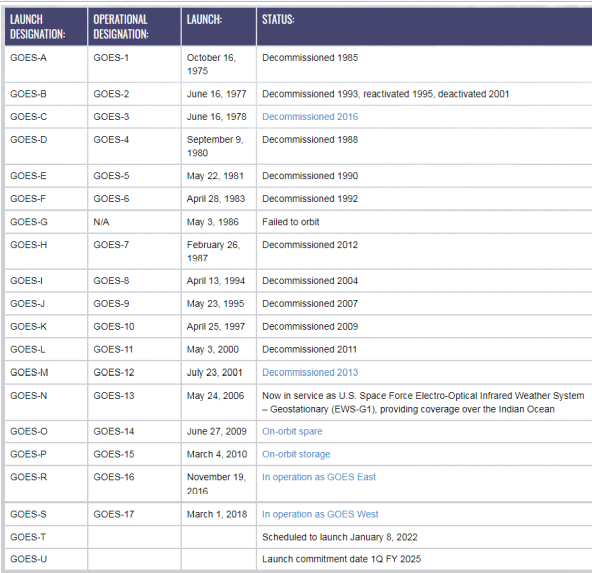
\includegraphics[scale=0.8]{image5.png} %\cite{umhe}
\end{center}
\caption{Goes-R Series}
\label{Goes-R Series}%\cite{ABIA}
\end{figure}
\section{GOES-R Series Instruments}
\paragraph{}
GOES-R Series has six instruments on board:
\begin{description}
\item[Earth-pointing] : 
\begin{itemize} 
\item Advanced Baseline Imager (ABI) - the primary instrument for imaging Earth’s weather, oceans and environment.
\item Geostationary Lightning Mapper (GLM) - a single-channel, near-infrared optical transient detector that can identify momentary changes in an optical scene, indicating the presence of lightning.
\end{itemize}
\item[Sun-pointing] : 
\begin{itemize} 
\item Extreme Ultraviolet and X-ray Irradiance Sensors (EXIS) - monitors solar irradiance in the upper atmosphere using two primary sensors: the Extreme Ultraviolet Sensor (EUVS) and the X-Ray Sensor (XRS).
\item  Solar Ultraviolet Imager (SUVI) - a telescope that monitors the sun in the extreme ultraviolet wavelength range, detecting solar flares and solar eruptions, and compiling full disk solar images.
\end{itemize}
\item[In-situ] : 
\begin{itemize} 
\item Magnetometer (MAG) - measures the space environment magnetic field that controls charged particle dynamics in the outer region of the magnetosphere
\item Space Environment In-Situ Suite (SEISS) - monitors proton, electron, and heavy ion fluxes in the magnetosphere using four sensors: the Energetic Heavy Ion Sensor (EHIS), the High and Low Magnetospheric Particle Sensors (MPS-HI and MPS-LO), and the Solar and Galactic Proton Sensor (SGPS).
\end{itemize}
\end{description}
\paragraph{}
Only two sensors are used for atmospheric purpose, Advanced Baseline Imager (ABI) and Geostationary Lightning Mapper (GLM).
\section{Advanced Baseline Imager (ABI)}

\paragraph{}
ABI is a multi-channel passive imaging radiometer that images Earth’s weather, oceans and environment with 16 spectral bands (2 visible, 4 near-infrared, and 10 infrared channels).

\begin{figure}[H]
\begin{center}
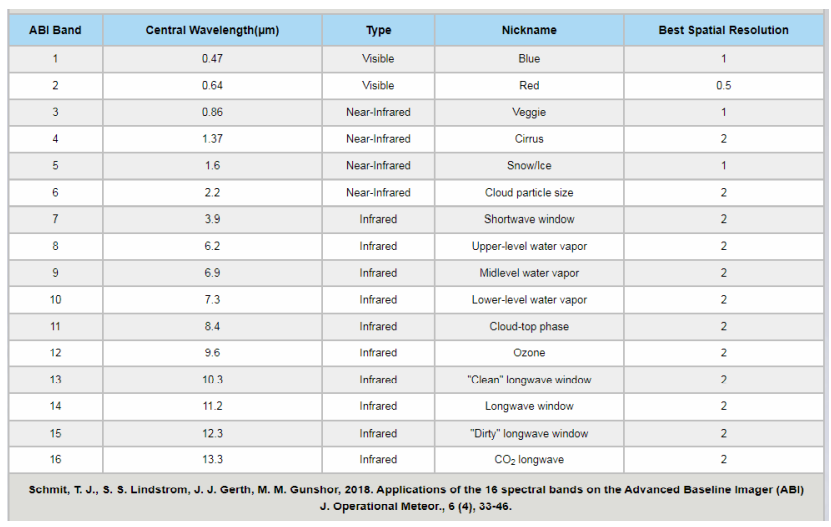
\includegraphics[scale=0.8]{abi_band_image.png} %\cite{umhe}
\end{center}
\caption{ABI optical components}
\label{ABI optical components}%\cite{ABIA}
\end{figure}
\section{ABI Data Collection Approach and Operations}
\paragraph{}
There are three major components of ABI that work together to collect observations of the Earth, space, and calibration targets as a system.
These are the scanning mirrors, the Four Mirror Anastigmat (FMA) telescope, and the Focal Plane Modules (FPMs).
\begin{figure}[H]
\begin{center}
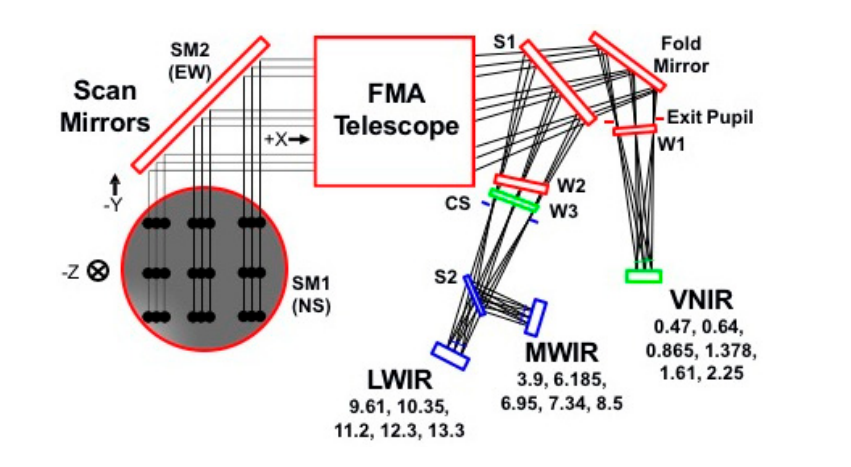
\includegraphics[scale=0.8]{abi_pos_image.png} %\cite{umhe}
\end{center}
\caption{ABI optical components}
\label{ABI optical components}%\cite{ABIA}
\end{figure}
\begin{flushleft}
	\begin{tabular}{lll}
	\textbf{SM}=Scan Mirror&\textbf{EW}=East–West&\textbf{NS}=North–South \\
	\vspace{0.5\baselineskip}
	\textbf{FMA}=Four Mirror Anastigmat&\textbf{S1, S2}=Beamsplitter 1 and 2 &\textbf{CS}=Cold Stop \\
	\vspace{ 0.5\baselineskip}
	\textbf{W1, W2, W3}=Windows 1, 2, and 3&\textbf{LWIR}=Longwave Infrared&\textbf{VNIR }=Visible and Near I\\
	\textbf{MWIR}=Mid-Wave IR&&\\
	\end{tabular}
\end{flushleft}
\section{ABI modes of operation}
\paragraph{}

\begin{description}
\item[Full Disk] : Hemispheric Coverage of 83° local zenith angle, temporal resolution of 5-15 minutes, and spatial resolution of 0.5 to 2km.
\item[ Mesoscale]: Provides coverage over a 1000x1000km box with a temporal resolution of 30 seconds, and spatial resolution of 0.5 to 2km.
\item[ Continental US/Pacific US]: The CONUS and PACUS scans are performed every five minutes, providing coverage of the 5000km (east/west) and 3000km (north/south) rectangle over the continental United States (GOES-16) or the Pacific Ocean, including Hawaii (GOES-17). The spatial resolution is 0.5 to 2km.
\item[ Flex Modes]: he flex modes provide a full disk scan every 10 minutes (mode 6) or every 15 minutes (mode 3), a CONUS/PACUS every five minutes, and two mesoscale domains every 60 seconds (or one sub-region every 30 seconds).
\end{description}
\section{GOES-R Data Products}
GOES-R Data products have three levels:
\begin{description}
\item [Level 0 (L0)] : are observation data received directly from the 6 satellite instruments. The data is not meaningful to most users prior to processing by the ground system.
\item [Level 1b (L1b)] : are calibrated and, where applicable, geographically corrected, L0 data. This means that the data has been processed so that its values are in standard units of physical quantities. For ABI, the L1b product is Radiances.
This is useful for users who require radiance units, instead of reflectance/brightness temperature (Kelvin) units.
All of the instruments have L1b products available except GLM, which is only distributed as an L2+ product.
\item [Level 2+ Products] : contain environmental physical qualities, such as cloud top height or land surface temperature.
Aside from the GLM Lightning Detection Product, the data source for these products is the ABI L1b data.
\end{description}
\section{ABI meteorological product}
The mission-critical ABI product is \href{https://www.goes-r.gov/products/baseline-cloud-moisture-imagery.html}{Cloud and Moisture Imagery} (CMI), which utilizes all 16 ABI spectral bands,
and is used to generate an array of products aiding forecasters in monitoring and predicting weather hazards.
The following is a list ABI meteorological and space weather data products that are available to the user community.
\begin{itemize} 
\item \href{https://www.goes-r.gov/products/baseline-aerosol-detection.html}{Aerosol detection (including smoke and dust)} 
\item \href{https://www.goes-r.gov/products/baseline-aerosol-opt-depth.html}{Aerosol optical depth (AOD)}
\item \href{https://www.goes-r.gov/products/opt2-aerosol-particle-size.html}{Aerosol particle size}
\item \href{https://www.goes-r.gov/products/baseline-clear-sky-mask.html}{Clear sky masks}
\item \href{https://www.goes-r.gov/products/opt2-cloud-layers-height.html}{Cloud layers/heights}
\item \href{https://www.goes-r.gov/products/baseline-cloud-moisture-imagery.html}{Cloud and moisture imagery}
\item \href{https://www.goes-r.gov/products/baseline-cloud-opt-depth.html}{Cloud optical depth}
\item \href{https://www.goes-r.gov/products/baseline-cloud-particle-size-dist.html}{Cloud particle size distribution}
\item \href{https://www.goes-r.gov/products/baseline-cloud-top-height-cloud-layer.html}{Cloud top height} 
\item \href{https://www.goes-r.gov/products/baseline-cloud-phase.html}{Cloud top phase}
\item \href{https://www.goes-r.gov/products/baseline-cloud-top-pressure.html}{Cloud top pressure}
\item \href{https://www.goes-r.gov/products/baseline-cloud-top-temp.html}{Cloud top temperature}
\item \href{https://www.goes-r.gov/products/baseline-derived-motion-winds.html}{Derived motion winds}
\item \href{https://www.goes-r.gov/products/baseline-derived-stability-indices.html}{Derived stability indices}
\item \href{https://www.goes-r.gov/products/baseline-DSR.html}{Downward shortwave radiation: surface}
\item \href{https://www.goes-r.gov/products/baseline-fire-hot-spot.html}{Fire/hot spot characterization}
\item \href{https://www.goes-r.gov/products/baseline-hurricane-intensity.html}{Hurricane intensity estimation}
\item \href{https://www.goes-r.gov/products/LSA.html}{Land surface albedo}
\item \href{https://www.goes-r.gov/products/BRF.html}{Land surface bidirectional reflectance factor}
\item \href{https://www.goes-r.gov/products/baseline-LST.html}{Land surface temperature (skin)}
\item \href{https://www.goes-r.gov/products/baseline-legacy-vert-moisture-profile.html}{Legacy vertical moisture profile}
\item \href{https://www.goes-r.gov/products/baseline-legacy-vert-temp-profile.html}{Legacy vertical temperature profile}
\item \href{https://www.goes-r.gov/products/baseline-radiances.html}{Radiances}
\item \href{https://www.goes-r.gov/products/baseline-rainfall-rate-qpe.html}{Rainfall rate/QPE}
\item \href{https://www.goes-r.gov/products/baseline-TOA.html}{Reflected shortwave radiation: TOA}
\item \href{https://www.goes-r.gov/products/opt2-sea-lake-ice-age.html}{Sea and lake ice: age}
\item \href{https://www.goes-r.gov/products/opt2-sea-lake-ice-concentration.html}{Sea and lake ice: concentration}
\item \href{https://www.goes-r.gov/products/opt2-sea-lake-ice-motion.html}{Sea and lake ice: motion}
\item \href{https://www.goes-r.gov/products/baseline-SST.html}{Sea surface temperature (skin)}
\item \href{https://www.goes-r.gov/products/baseline-snow-cover.html}{Snow cover}
\item \href{https://www.goes-r.gov/products/baseline-total-precipitable-water.html}{Total precipitable water}
\item \href{https://www.goes-r.gov/products/baseline-volcanic-ash.html}{Volcanic ash: detection and height}
\end{itemize}



\newpage

ls
%\chapter{\normalsize{BACKGROUND OF SATELLITE REMOTE SENSING}}
\chapter{\normalsize{SATELLITE DATA ANALYSIS}}
\section{Technique 1: access data files}
\subsection{Access data files from NOAA CLASS}
\begin{itemize} 
\item The NOAA \href{https://www.avl.class.noaa.gov/saa/products/welcome}{Comprehensive Large Array-data Stewardship System (CLASS)} repository is the official site for accessing all available GOES-R Series Products.
\item  A similar but easier website to navigate is NCEI's Archive \href{https://www.ncdc.noaa.gov/airs-web/search}{Archive Information Request System (AIRS)}.
\end{itemize}
\subsection{Access data files from Amazon, Microsoft, OCC}
\begin{itemize}
\item \href{https://registry.opendata.aws/noaa-goes/}{Amazon Web Service (AWS)} - ABI L1b and L2+, GLM L2+, and SUVI L1b products are available in AWS S3 Buckets. These open datasets can be accessed by the public from AWS for free. 
\item \href{https://azure.microsoft.com/en-us/services/open-datasets/catalog/goes-16/}{Microsoft Azure}  - Two GOES-16 ABI Full Disk products are stored in a Azure blob container. 
The products currently available are L1b Radiances and L2+ MCMI, which can be accessed from Azure for free.
\item  \href{http://edc.occ-data.org/goes16/}{Open Commons Consortium (OCC)} - Stores a 100 TB rolling archive of GOES-16 data (\~{}8 months), the products stored are ABI L1b and ABI L2+ CMI and MCMI. OCC recommends using the AWS CLI or the python boto library, to access the data. 
\end{itemize}
\subsection{Access data files from Google Cloud}
\begin{itemize}
\item \href{https://console.cloud.google.com/marketplace/product/noaa-public/goes-16?filter=category:science-research&id=5babd633-afa0-4e40-9dba-0587f4aabc47}{Google Cloud} - ABI L1b and L2+, GLM L2+, and SUVI L1b products are available in two different buckets for GOES-16 and GOES-17. 
\item \href{https://developers.google.com/earth-engine}{Google Earth Engine (GEE)} - A cloud-based platform for geospatial analysis. This service runs through 
Google Cloud, and pulls GOES-R datasets from the Google Cloud buckets. 
\end{itemize}
\subsection{Use Python to retrieve data from AWS}
Python is the most powerful programming language using in data science and geospatial data analysis.
The following sample scripts demonstrate how to retrieve GOES-R files from AWS using  Python. 
\begin{lstlisting}[language=Python]
from goespy.Downloader import ABI_Downloader
### to use ABI_Downloader, you need 7 arguments:
import datetime as dt 
### Getting the current date (in UTC coordinate)
utcDateTime = dt.datetime.utcnow() 
## current year
year = utcDateTime.strftime("%Y")
# current month
month = utcDateTime.strftime("%m")
## current day
day = utcDateTime.strftime("%d")
## current hour in UTC 
hour = utcDateTime.strftime("%H")
##Choose a channel from your preference (can be C01-C16)
channel = ["C01"]
## In GOES satellite they have 9 products
## 3 are L1b-Rad(M,C,F)
## 3 are L2-CMIP(M,C,F)
## 3 are L2-MCMIP(M,C,F)
### In your case we will get the CMIPF, F means FullDisk (all the projection by the satellite)
product = 'L1b-L2-CMIPF'
## The Bucket is the variable contains the name of dataset server from goes on AWS
Bucket = 'noaa-goes16' ## in the future on AWS they will have goes17.
## Now we will call the function ABI_Downloader:
Abi = ABI_Downloader('noaa-goes16',year,month,day,hour,product,channel)
\end{lstlisting}
After all the dataset is downloaded, they are in your home directory with that structure:
\begin{figure}[H]
\begin{center}
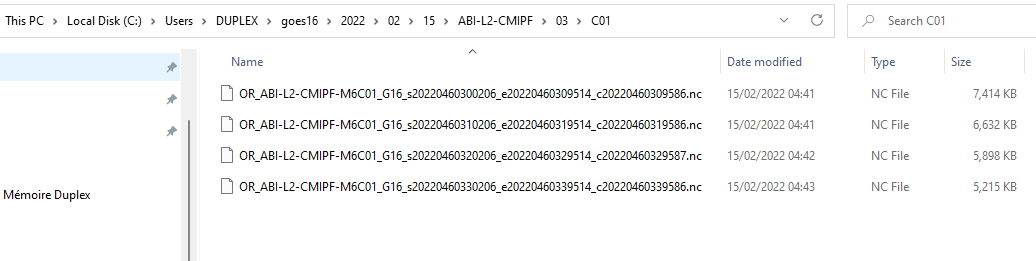
\includegraphics[scale=0.8]{file1.png} %\cite{umhe}
\end{center}
\caption{L1b-L2-CMIPF product downloaded}
\label{L1b-L2-CMIPF product downloaded}%\cite{ABIA}
\end{figure}
\section{Technique 2: Explore satellite data and metadata}
\subsection{ GOES-R Series data format}
GOES-R Series product files use the netCDF-4 format.
NetCDF (Network Common Data Form) is a set of software libraries and machine-independent data formats that support the creation, access, and sharing of array-oriented scientific data. It is also a community standard for sharing scientific data.
\subsection{Read metadata}
Metadata provides information about the distinct items, such as: means of creation, purpose of 
the data, time and date of creation, creator or author of data, placement on a network (electronic 
form) where the data was created, what standards used etc.
The main purpose of metadata is to facilitate in the discovery of relevant information, more often 
classified as resource discovery. Metadata also helps organize electronic resources, provide 
digital identification, and helps support archiving and preservation of the resource.
Before any manipulation of data, it is vitaly important to read metadata.
Now let us see how to read the metadata of this satellite data file in command line using gdal tools.
\begin{lstlisting}[language=Bash]
## change directory to where you have downloaded the GLDAS data using the below
cd /mnt/d/MI_IS_DATA_ANALYSIS
## extatract metadata of the 'OR_ABI-L1b-RadM1-M3C02_G16_s20171931811268_e20171931811326_c20171931811356.nc' 
gdalinfo OR_ABI-L1b-RadM1-M3C02_G16_s20171931811268_e20171931811326_c20171931811356.nc
## press enter
\end{lstlisting}
\begin{figure}[H]
\begin{center}
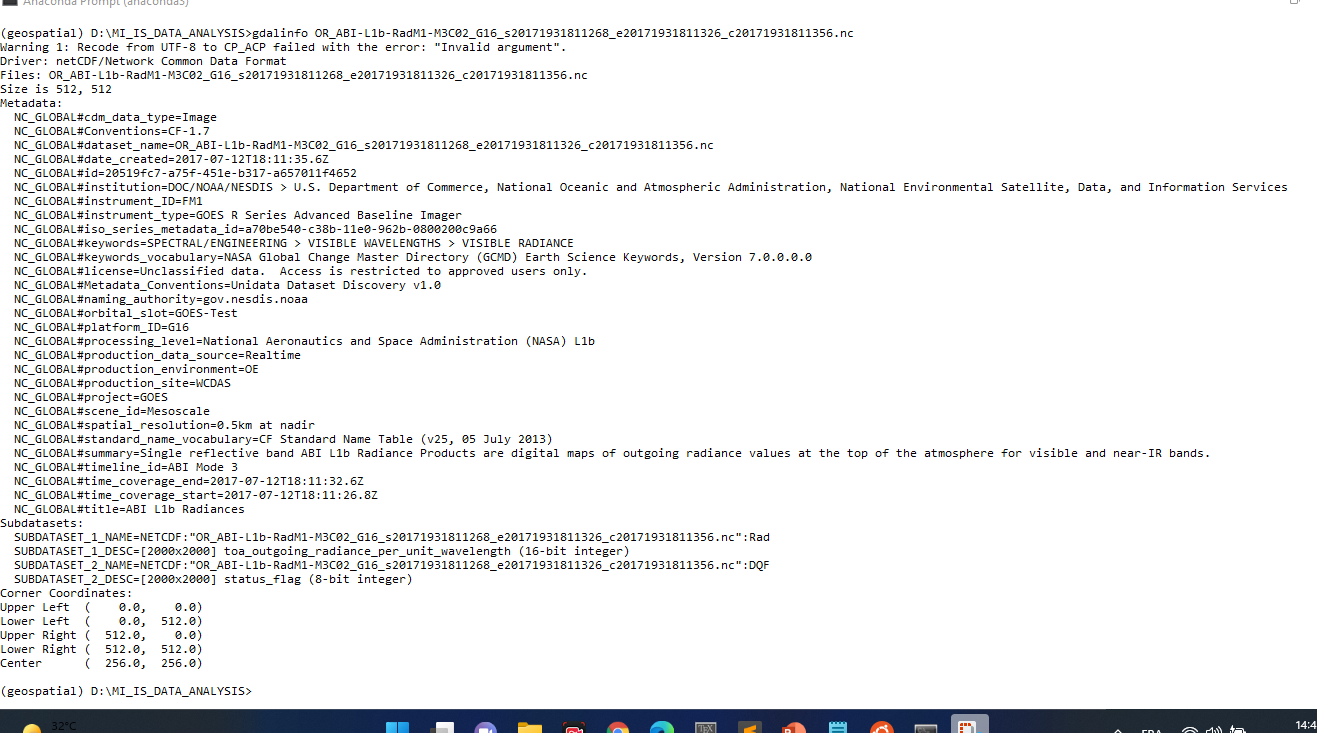
\includegraphics[scale=0.5]{gdal1.png} %\cite{umhe}
\end{center}
\caption{metadata}
\label{metadta}%\cite{ABIA}
\end{figure}

\section{Technique 3: Plot a single band ABI Channel}
ABI imager has 16 channels, the code below show how to plot a single band ABI channel.
\begin{lstlisting}[language=Python]
def open_dataset(date, channel, idx, region):
    """
    Open and return a netCDF Dataset object for a given date, channel, and image index
    of GOES-16 data from THREDDS test server.
    """
    cat = TDSCatalog('https://thredds.ucar.edu/thredds/catalog/satellite/goes/east/products/'
                     f'CloudAndMoistureImagery/{region}/Channel{channel:02d}/{date:%Y%m%d}/catalog.xml')
    ds = cat.datasets[idx]
    ds = ds.remote_access(use_xarray=True)   
    return ds
def plot_GOES16_channel(date, idx, channel, region):
    """
    Get and plot a GOES 16 data band from the ABI.
    """
    ds = open_dataset(date, channel, idx, region)
    dat = ds.metpy.parse_cf('Sectorized_CMI')
    proj = dat.metpy.cartopy_crs
    x = dat['x']
    y = dat['y']
    fig = plt.figure(figsize=(10, 10))
    ax = fig.add_subplot(1, 1, 1, projection=proj)
    ax.add_feature(cfeature.COASTLINE, linewidth=2)
    ax.add_feature(cfeature.STATES, linestyle=':', edgecolor='black')
    ax.add_feature(cfeature.BORDERS, linewidth=2, edgecolor='black')
    for im in ax.images:
        im.remove()
    im = ax.imshow(dat, extent=(x.min(), x.max(), y.min(), y.max()), origin='upper')
    timestamp = datetime.strptime(ds.start_date_time, '%Y%j%H%M%S')
    add_timestamp(ax, time=timestamp, high_contrast=True, 
                  pretext=f'GOES 16 Ch.{channel} - ',
                  time_format='%d %B %Y %H%MZ', y=0.01,
                  fontsize=18)
    display(fig)
    plt.savefig("goes_fulldisk_C1.png")
    plt.close()
channel_list = {u'1 - Blue Band 0.47 \u03BCm': 1,
                u'2 - Red Band 0.64 \u03BCm': 2,
                u'3 - Veggie Band 0.86 \u03BCm': 3,
                u'4 - Cirrus Band 1.37 \u03BCm': 4,
                u'5 - Snow/Ice Band 1.6 \u03BCm': 5,
                u'6 - Cloud Particle Size Band 2.2 \u03BCm': 6,
                u'7 - Shortwave Window Band 3.9 \u03BCm': 7,
                u'8 - Upper-Level Tropo. WV Band 6.2 \u03BCm': 8,
                u'9 - Mid-Level Tropo. WV Band 6.9 \u03BCm': 9,
                u'10 - Low-Level WV Band 7.3 \u03BCm': 10,
                u'11 - Cloud-Top Phase Band 8.4 \u03BCm': 11,
                u'12 - Ozone Band 9.6 \u03BCm': 12,
                u'13 - Clean IR Longwave Band 10.3 \u03BCm': 13,
                u'14 - IR Longwave Band 11.2 \u03BCm': 14,
                u'15 - Dirty Longwave Band 12.3 \u03BCm': 15,
                u'16 - CO2 Longwave IR 13.3 \u03BCm': 16}
region = Select(
    options=['Mesoscale-1', 'Mesoscale-2', 'CONUS', 'PuertoRico', 'FullDisk'],
    description='Region:',)

channel = Dropdown(options=channel_list,value=16,description='Channel:',)

interact(plot_GOES16_channel, date=fixed(date), idx=fixed(-2), 
         channel=channel, region=region)

\end{lstlisting}

\begin{figure}[h!]
%\begin{figure}[H]
%\begin{figure}[t]
%\begin{figure}[b]
%\begin{figure}[b]
  \centering
  \begin{subfigure}[a]{0.4\linewidth}
    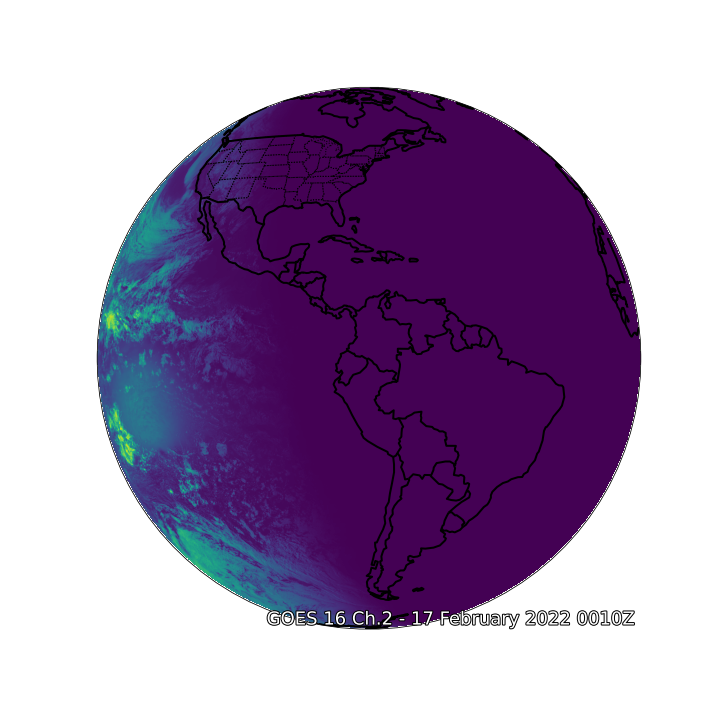
\includegraphics[width=\linewidth]{goes_fulldisk_C01.png}
     \caption{ABI CH01}
  \end{subfigure}
   %\centering
  \begin{subfigure}[b]{0.4\linewidth}
    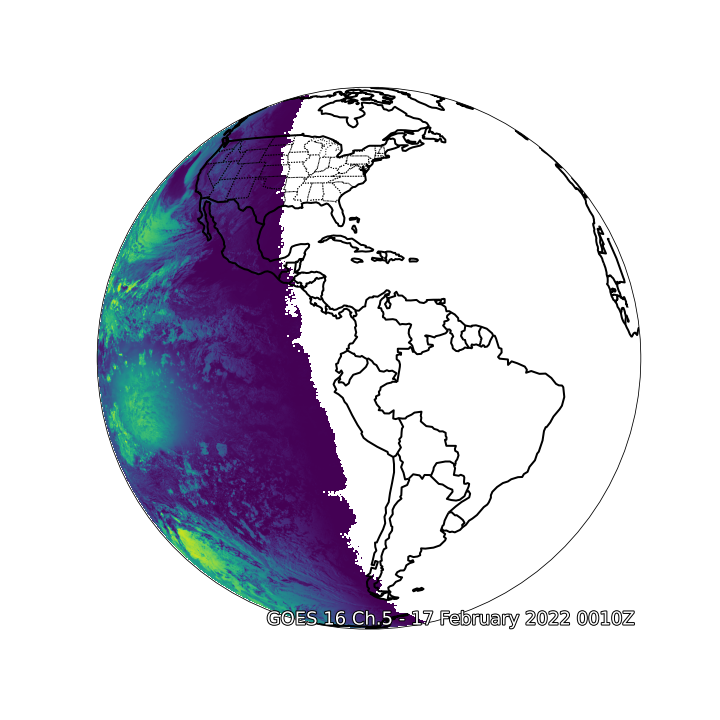
\includegraphics[width=\linewidth]{goes_fulldisk_C05.png}
    \caption{ABI CH05}
  \end{subfigure}
   %\centering
  \begin{subfigure}[b]{0.4\linewidth}
    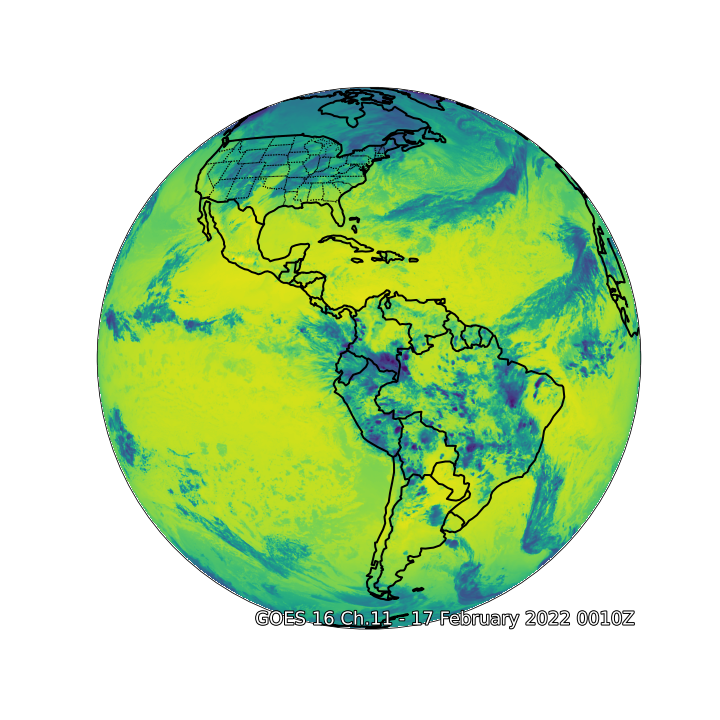
\includegraphics[width=\linewidth]{goes_fulldisk_C11.png}
    \caption{ABI CH11}
  \end{subfigure}
   %\centering
  \begin{subfigure}[b]{0.4\linewidth}
    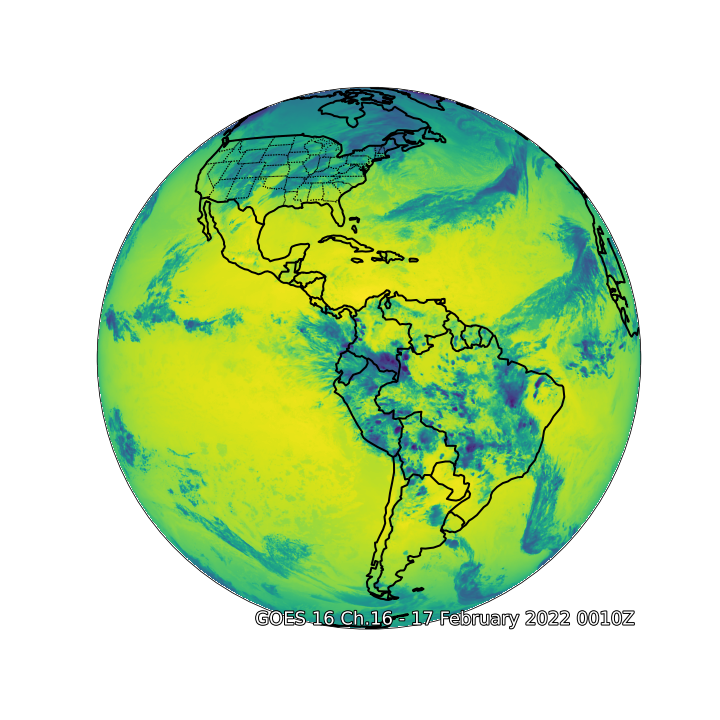
\includegraphics[width=\linewidth]{goes_fulldisk_C16.png}
    \caption{ABI CH16}
  \end{subfigure}
  \caption{ABI BAND SAMPLE PLOT}
  \label{ABI BAND SAMPLE PLOT}
\end{figure}



\section{Convert NetCDF files to GeoTIFFs }
GeoTIFFS are regarded as the industry standard for georeferenced raster data.
The conversion of GOES-R netCDF arrays to single-band GeoTIFF rasters can be 
accomplished in command line. This conversion is very usefull because GeoTIFFS data format are easy to inject in Geographic Information System (GIS) software like QGIS.
\begin{lstlisting}[language=Bash]
##  Convert radiance from NetCDF files to GeoTIFF - below command
gdal_translate NETCDF:"OR_ABI-L1b-RadM1-M3C02_G16_s20171931811268_e20171931811326_c20171931811356.nc":OR_ABI-L1b-RadM1-M3C02_G16_s20171931811268_e20171931811326_c20171931811356.tif
\end{lstlisting}

\section{Technique 5: Processing satellite data using GIS Software}
\subsection{Objectives}
The main objective of this analysis is to process satellite data and compare with data obtained from at aeronautical met stations. Here we will use the three hour data from  \href{https://ldas.gsfc.nasa.gov/gldas}{GLDAS}.
\subsection{Avition meteorological stations in cameroon}


\begin{table}[H]
\caption{Aviation meteorological stations}
\label{tab:Aviation meteorological stations}
\begin{center}
\begin{tabular}{| l | c | c | c | c |}
\hline
\textbf{NAME} & \textbf{OMM CODE} & \textbf{ICAO CODE} & \textbf{LATITUDE} & \textbf{LONGITUDE}\\[2pt] \hline
Yaounde	& 64950&	FKYS&	03°50N&	011°31E \\\hline
Douala	& 64910	& FKKD	& 04°00N& 	009°44E \\\hline
Garoua	& 64860& 	FKKR& 	09°20N& 	013°23E\\\hline
Maroua	& 64851	& FKKL& 	10°27’N	& 14°15’E\\\hline
Ngaoundéré& 	64870& 	FKKN& 	07°21N& 013°34E\\\hline
Bafoussam& 	64894& 	FKKU& 	05°32’05 N& 	010°21’15 E\\\hline
Bertoua& 	64930& 	FKKO& 	04°36N& 	013°44E\\\hline
Bamenda& 	64892& 	FKKV& 	06°03N& 	010°07E\\\hline
\end{tabular}
\end{center}
\end{table}


\begin{figure}[H]
\begin{center}
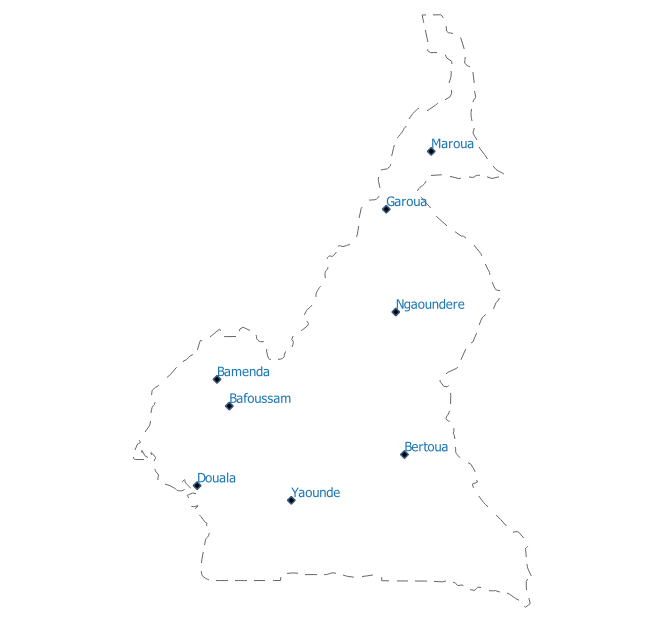
\includegraphics[scale=0.8]{cmr_station.png} %\cite{umhe}
\end{center}
\caption{aviation meteorological stations}
\label{aviation meteorological stations}%\cite{ABIA}
\end{figure}
\subsection{GLDAS data}
The goal of the Global Land Data Assimilation System (GLDAS) is to ingest satellite- and ground-based observational data products, using advanced land surface modeling and data assimilation techniques, in order to generate optimal fields of land surface states and fluxes (Rodell et al., 2004a).
GLDAS data are available to download from this \href{https://hydro1.gesdisc.eosdis.nasa.gov/data/GLDAS/GLDAS_NOAH025_3H.2.1/}{link}.
Detailed documentation about GLDAS 2.1 product is available \href{https://hydro1.gesdisc.eosdis.nasa.gov/data/GLDAS/GLDAS_NOAH025_3H.2.1/doc/README_GLDAS2.pdf.}{here}  

\subsection{Specific requirements}
The requirements for the metereorological data at aeronautical station are:
\begin{figure}[H]
\begin{center}
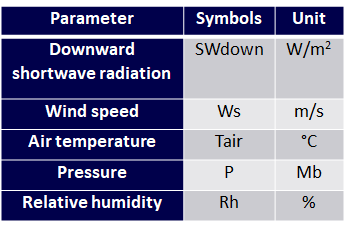
\includegraphics[scale=0.8]{gldas1.png} %\cite{umhe}
\end{center}
\caption{meteorological data required}
\label{meteorological data required}%\cite{ABIA}
\end{figure}
The units at which GLDAS provide air temperature (K) and Pressure(Pa). Further GLDAS provide specific humidity. 
To match requirements the following conversion steps have to be performed:
\begin{description}
\item[Step 1] : Convert GLDAS air temperature from Kelvin to Deg C.
\item[Step 2] : Convert the unit of GLDAS pressure from Pa to Milli bar (Mb).
\item[Step 3] : Convert specific humidity to relative humidity following the description \href{https://earthscience.stackexchange.com/questions/2360/how-do-i-convert-specific-humidity-to-relative-humidity/}{here}.
\item[Step 4] : Extract the Ws, Tair, P and Rh corresponding at our aeronautical meteorological stations at observation time : 00:00, O3:00, O6:00, 09:00, 12:00, 15:00, 18:00 and 21:00 UTC.
\item[Step 5] : Compare the results with data collected at the stations.
\end{description}
\subsection{Download GLDAS data}
To download GLDAS data, we can use python script as shown below.
\begin{lstlisting}[language=Bash]
## In the Ubuntu session.
## Type in the following command to install the python package "gldas"
pip3 install gldas
## press enter
## Below code will download the GLDAS data between the dates provided in the command.
gldas_download -s 2021-01-01 -e 2021-01-31 --product GLDAS_Noah_v21_025 --username nina.younkap --password ****** /mnt/path/to/folder
## Note that the last argument in above command is path to a folder where the downloaded files will be stored.
\end{lstlisting}
\subsection{Processing single data file}
Let us now see how to process a single NetCDF file (.nc4) dowloaded from GLDAS using the previous step and perform the required conversions.
For example let us consider the GLDAS data representing 06:00 hours on 31 January 2021.
The GLDAS file name follows a particular structure.
\newline
The file name is \textbf{GLDAS\_NOAH025\_3H.A20210131.0600.021.nc4}
\begin{itemize}
\item \textcolor{magenta}{GLDAS\_NOAH025\_3H} represents the name, spatial resolution (025 means 0.25 degree resolution) and temporal resolution (3H means three hour data)
\item \textcolor{magenta}{A20210131}  represents the date of acquisition
\item \textcolor{magenta}{0600}  represents the time (in this case 06:00 GMT) the parameters are computed for.
\item \textcolor{magenta}{021}  represents the version of GLDAS data, in this case 2.1.
\item \textcolor{magenta}{nc4}  represents the extension and format of the data, in this case netCDF4.
\end{itemize}
Now let us see how to read the metadata of this file in command line using gdal tools
\begin{lstlisting}[language=Bash]
## change directory to where you have downloaded the GLDAS data using the below
cd /mnt/d/mi_is_project_data/2021/31"
## Extract metadata of the 'GLDAS_NOAH025_3H.A20210131.0600.021.nc4' in the file "metadata.txt"
gdalinfo GLDAS_NOAH025_3H.A20210131.0600.021.nc4 > metadata.txt
## press enter
## Read metadata using vim editor
vim metadata.txt
\end{lstlisting}
In the metadata, under Subdatasets: all the parameters provided as subdatasets are listed. 
These subdataset names are used in the further steps to process individual parameters. For example, NETCDF:\textcolor{magenta}{"GLDAS\_NOAH025\_3H.A20210131.0600.021.nc4":Tair\_f\_inst} is the name of air temperature grid at 06:00 on 31 January 2021 and we will use this name to extract/process this single grid. 
The codes of the parameters are listed in the \href{https://hydro1.gesdisc.eosdis.nasa.gov/data/GLDAS/GLDAS_NOAH025_3H.2.1/doc/README_GLDAS2.pdf}{GLDAS user manual} (Table 3.1).
\newline
So for our project we need the following subdatasets from a single GLDAS file:
\newline
\vspace{0.5\baselineskip}
\textcolor{magenta}{NETCDF:"GLDAS\_NOAH025\_3H.A20210131.0600.021.nc4":Qair\_f\_inst} - Specific humidity (Kg/Kg)
\newline
\vspace{0.5\baselineskip}
\textcolor{magenta}{NETCDF:"GLDAS\_NOAH025\_3H.A20210131.0600.021.nc4":Psurf\_f\_inst} - Surface Pressure (Pa)
\newline
\vspace{0.5\baselineskip}
\textcolor{magenta}{NETCDF:"GLDAS\_NOAH025\_3H.A20210131.0600.021.nc4":Tair\_f\_inst} - Air Temperature (K)
\newline
\vspace{0.5\baselineskip}
\textcolor{magenta}{NETCDF:"GLDAS\_NOAH025\_3H.A20210131.0600.021.nc4":Wind\_f\_inst } - Wind speed (m/s)
\newline
\vspace{0.5\baselineskip}
\textcolor{magenta}{NETCDF:"GLDAS\_NOAH025\_3H.A20210131.0600.021.nc4":SWdown\_f\_inst} - Downward short-wave radiation flux (W m-2)
\newline
Now let us extract each of the above subdatasets and convert them into tif file. For this we will use a gdal command called \textcolor{magenta}{gdal\_translate} which is a global conversion tool for all kind of raster formats. Detailed documentation on gdal\_translate is given \href{https://gdal.org/programs/gdal_translate.html}{here}.
\begin{lstlisting}[language=Bash]
##  Convert specific humidity to tif - below command
gdal_translate NETCDF:"GLDAS_NOAH025_3H.A20210131.0600.021.nc4":Qair_f_inst GLDAS_NOAH025_3H_A20210131_0600_Qair.tif
## Convert Surface Pressure to tif - below command
gdal_translate NETCDF:"GLDAS_NOAH025_3H.A20210131.0600.021.nc4":Psurf_f_inst GLDAS_NOAH025_3H_A20210131_0600_Psurf.tif
## Convert air temperature to tif - below command
gdal_translate NETCDF:"GLDAS_NOAH025_3H.A20210131.0600.021.nc4":Tair_f_inst GLDAS_NOAH025_3H_A20210131_0600_Tair.tif
## Convert Wind speed to tif - below command
gdal_translate NETCDF:"GLDAS_NOAH025_3H.A20210131.0600.021.nc4":Wind_f_inst GLDAS_NOAH025_3H_A20210131_0600_Wind.tif
## Convert Short wave downward radiation to tif - below command
gdal_translate NETCDF:"GLDAS_NOAH025_3H.A20210131.0600.021.nc4":SWdown_f_tavg GLDAS_NOAH025_3H_A20210131_0600_SWdown.tif
## Press enter
\end{lstlisting}
Now that we have the required parameters of 31 January 2021 in tif format, let us open the air temperature map in QGIS and see how it looks!
\begin{figure}[H]
\begin{center}
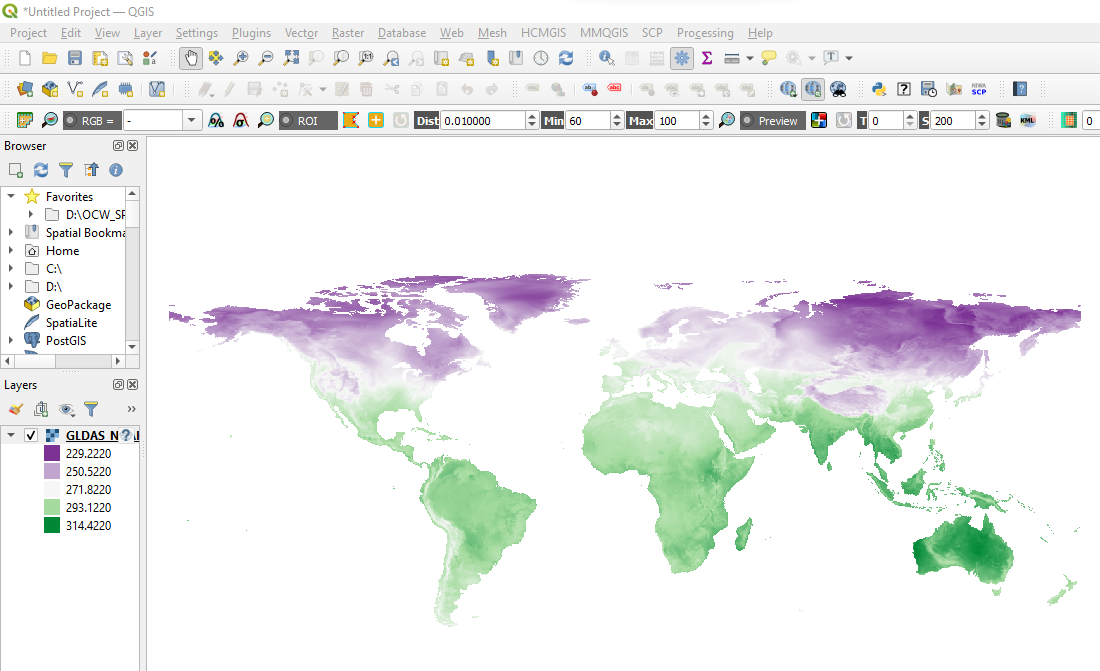
\includegraphics[scale=0.6]{qgis1.png} %\cite{umhe}
\end{center}
\caption{GLDAS Tair data displayed in QGIS}
\label{GLDAS Tair data displayed in QGIS}%\cite{ABIA}
\end{figure}
\paragraph{}
Let us also zoom to Cameroon boundaries and have a look at the Tair map.
Remember the resolution of data is 0.25 degrees.
\begin{figure}[H]
\begin{center}
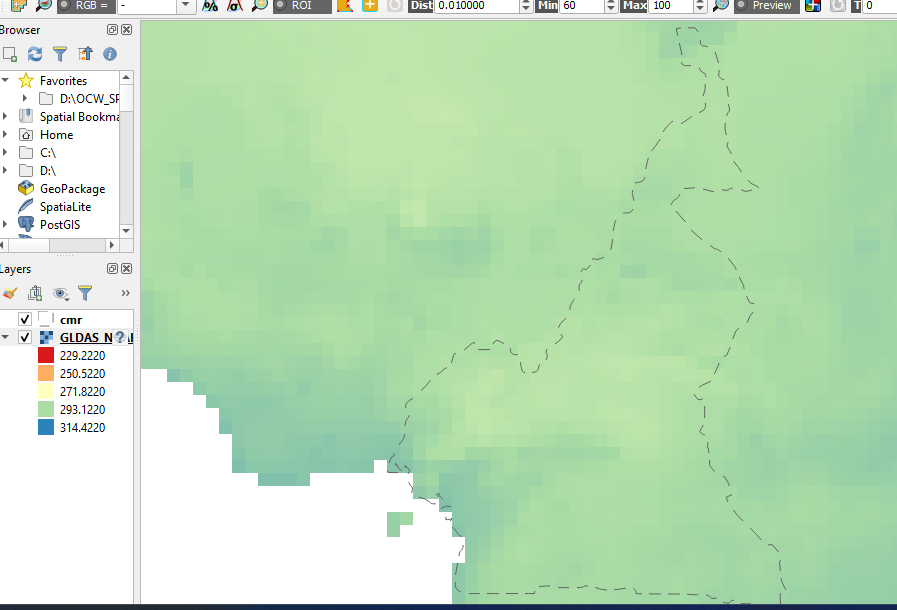
\includegraphics[scale=0.6]{qgis2.png} %\cite{umhe}
\end{center}
\caption{GLDAS Tair data displayed in QGIS and zoomed to Cameroon}
\label{GLDAS Tair data displayed in QGIS and zoomed to Cameroon}%\cite{ABIA}
\end{figure}
Now let us see how to do unit conversion of all the five parameters required for aviation. 
One additional step is to clip the unit converted maps to cameroon boundaries as we are only interested in that region not global.
\newline
For further steps let us move to \textcolor{magenta}{GRASS GIS} as it is easier to do spatial and temporal analysis with GRASS library. 
We will create a new location and mapset for processing GLDAS data for Cameroon.
\begin{lstlisting}[language=Bash]
# Create (-c) just the location called "cmr" in epsg:4326 and exit (-e)
grass78 epsg:4326 /mnt/d/grassdata/cmr -c -e
# Create (-c) mapset called "met_data" inside the location "cmr" and open GRASS GIS in "cmr/met_data" mapset
grass78 /mnt/d/grassdata/cmr/met_data -c
# "-c" flag in above command is required only one time to create the mapset met_data
# Afterwards use below command to just start the existing mapset.
# grass78 /mnt/d/grassdata/cmr/met_data
\end{lstlisting}
Import the cameroon vector file , aviation meteorological station file , and others file required for our project into grass location. 
\begin{lstlisting}[language=Bash]
## IMPORT VECTOR DATA: Boundaries of Cameroon an  Aviation meteorological station in cameroon
## Navigate (cd) to the folder Cmr_Base_Layers
cd /mnt/d/mi_is_project_data/Cmr_Base_Layers 
# Import 'Cameroon' boundary shapefile into a vector in Grass GIS
v.import in=cmr.shp out=cmr
# Import 'Aviation meteorological staitions' points shapefile into a vector in Grass GIS
v.import in=aero_met_station_cmr.shp out=met_station
# Import 'FKKR TMA2' boundary shapefile into a vector in Grass GIS
v.import in=Fkkr_tma2.shp out=fkkr_tma2
# Import 'FKKN TMA' boundary shapefile into a vector in Grass GIS
v.import in=Fkkn_tma.shp out=fkkn_tma
# Import 'FKKL CONTROL ZONE' boundary shapefile into a vector in Grass GIS
v.import in=Fkkl_ctr.shp out=fkkl_ctr
# set the computational region to Cameroon Boundaries and set the computational resolution to 0.25 degrees
g.region vector=cmr res=0.25 -a
\end{lstlisting}
To automate the workflows, the following bash script process all the 5 required parameters (Tair, Rh, Wind speed, Psurf and SWDown), clipped on cameroon boundaries  and converted to the required units from .nc4 files in a day.
\begin{lstlisting}[language=Bash]
#!/bin/bash
## This script process a single day GLDAS data and do all the required conversions needed for our project.
## GENERAL ##
if [ -z "$GISBASE" ] ; then
    echo "You must be in GRASS GIS to run this program." >&2
    exit 1
fi
# Set a environment to enable overwrite by default
export GRASS_OVERWRITE=1

# Navigate to the folder containing single day .nc4 files
#e.g INDAT="/mnt/d/mi_is_project_data/Cmr_Base_Layers/2021/01" for 01 January 2021
#Here we work on the  31 January 2021 data
INDAT="/mnt/d/mi_is_project_data/2021/031" 
cd ${INDAT}
# set the computational region to Urmia Lake basin and set the computational resolution to 0.25 degrees
g.region vector=cmr res=0.25 -a
# set the mask to cameroon boundaries
#r.mask vect=cmr

# For loop to process all the .nc files in one go
for i in `ls GLDAS*.nc4`; do
    dt=`echo ${i}|cut -d. -f2-3`
    #  Convert specific humidity to tif - below command
    gdal_translate NETCDF:"${i}":Qair_f_inst GLDAS_NOAH025_3H_${dt}_Qair.tif
    # Convert Surface Pressure to tif - below command
    gdal_translate NETCDF:"${i}":Psurf_f_inst GLDAS_NOAH025_3H_${dt}_Psurf.tif
    # Convert air temperature to tif - below command
    gdal_translate NETCDF:"${i}":Tair_f_inst GLDAS_NOAH025_3H_${dt}_Tair.tif
    # Convert Wind speed to tif - below command
    gdal_translate NETCDF:"${i}":Wind_f_inst GLDAS_NOAH025_3H_${dt}_Wind.tif
    # Convert Short wave downward radiation to tif - below command
    gdal_translate NETCDF:"${i}":SWdown_f_tavg GLDAS_NOAH025_3H_${dt}_SWdown.tif
    # Import to GRASS
    # Import and clip specific humidity
    r.import in=GLDAS_NOAH025_3H_${dt}_Qair.tif out=GLDAS_NOAH025_3H_${dt}_Qair -o
    # Import and clip Surface Pressure
    r.import in=GLDAS_NOAH025_3H_${dt}_Psurf.tif out=GLDAS_NOAH025_3H_${dt}_Psurf -o
    # Import and clip Tair
    r.import in=GLDAS_NOAH025_3H_${dt}_Tair.tif out=GLDAS_NOAH025_3H_${dt}_Tair -o
    # Import and clip Wind speed
    r.import in=GLDAS_NOAH025_3H_${dt}_Wind.tif out=GLDAS_NOAH025_3H_${dt}_Wind -o
    # Import and clip Short wave radiation
    r.import in=GLDAS_NOAH025_3H_${dt}_SWdown.tif out=GLDAS_NOAH025_3H_${dt}_SWdown -o
    # Unit conversion
    # Air temperature from Kelvin to degree celsius
    r.mapcalc "GLDAS_NOAH025_3H_${dt}_Tair_final = GLDAS_NOAH025_3H_${dt}_Tair - 273.15"
    # Short wave radiation (no conversion required)
    r.mapcalc "GLDAS_NOAH025_3H_${dt}_SWdown_final = GLDAS_NOAH025_3H_${dt}_SWdown"
    # Wind speed (no conversion required)
    r.mapcalc "GLDAS_NOAH025_3H_${dt}_Wind_final = GLDAS_NOAH025_3H_${dt}_Wind"
    ## Specific humidity re saved
    r.mapcalc "GLDAS_NOAH025_3H_${dt}_Qair_final = GLDAS_NOAH025_3H_${dt}_Qair"
    ## Pressure convert from pa to mb
    r.mapcalc "GLDAS_NOAH025_3H_${dt}_Psurf_final = GLDAS_NOAH025_3H_${dt}_Psurf / 100"
    ## Humidity according to the url: https://earthscience.stackexchange.com/questions/2360/how-do-i-convert-specific-humidity-to-relative-humidity
    r.mapcalc "es = 6.112 * exp((17.67 * GLDAS_NOAH025_3H_${dt}_Tair_final) / (GLDAS_NOAH025_3H_${dt}_Tair_final + 243.5))"
    r.mapcalc "e = (GLDAS_NOAH025_3H_${dt}_Qair_final * GLDAS_NOAH025_3H_${dt}_Psurf_final) / (0.378 * GLDAS_NOAH025_3H_${dt}_Qair_final + 0.622)"
    r.mapcalc "GLDAS_NOAH025_3H_${dt}_Rh = (e / es) * 100"
    # Final Relative humidity in %
    r.mapcalc "GLDAS_NOAH025_3H_${dt}_Rh_final = float(if(GLDAS_NOAH025_3H_${dt}_Rh > 100, 100, if(GLDAS_NOAH025_3H_${dt}_Rh < 0, 0, GLDAS_NOAH025_3H_${dt}_Rh)))"

done
# Remove the mask
#r.mask -r
\end{lstlisting}
We save the script above in the file \textit{myscript.sh}. The following script show how to run this file on Linux Operating System.
\begin{lstlisting}[language=Bash]
# Run the following command to install dos2unix
sudo apt-get install dos2unix
# Below command removes the trailing spaces from your script
dos2unix myscript.sh
# Run the following command to run the above saved script file
sh myscript.sh
# press enter
\end{lstlisting}
\subsection{Results}
\subsection{Temperature chart}
\begin{lstlisting}[language=Bash]
#dt="20210131.0300"
dt="20210131.1500"
# Visualize data
r.mask vect=cmr --o
# Open a monitor
d.mon wx0
# Display a raster map
d.rast GLDAS_NOAH025_3H_A${dt}_Tair_final
# Display a vector map
d.vect map=cmr type=boundary
d.text text="31 JAN 2021 0300Z" color=black bgcolor=white size=3
# Add raster legend
d.legend -t -s -b raster=GLDAS_NOAH025_3H_A${dt}_Tair_final title=TEMPERATURE title_fontsize=20 font=sans fontsize=18
# Add North arrow
d.northarrow style=1b text_color=black
#Clear the monitor
#d.erase -f
#r.mask -r
# press enter
\end{lstlisting}

\begin{figure}[H]
\begin{center}
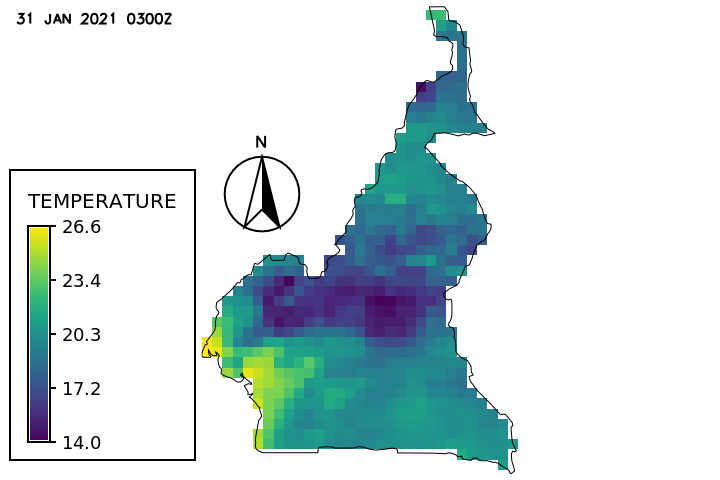
\includegraphics[scale=0.8]{tp03.png} %\cite{umhe}
\end{center}
\caption{Temperature at 03:00 UTC}
\label{Temperature at 03:00 UTC}%\cite{ABIA}
\end{figure}

\begin{figure}[H]
\begin{center}
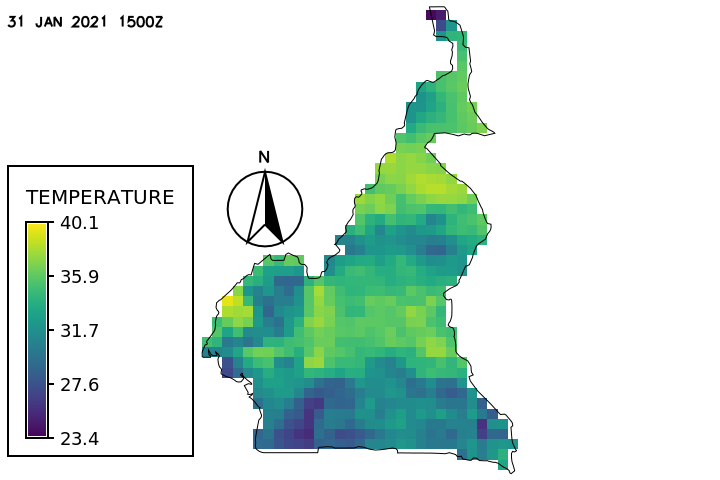
\includegraphics[scale=0.8]{tp15.png} %\cite{umhe}
\end{center}
\caption{Temperature at 15:00 UTC}
\label{Temperature at 15:00 UTC}%\cite{ABIA}
\end{figure}

\subsection{Relative Humidity Chart}
\begin{lstlisting}[language=Bash]
dt="20210131.0300"
#dt="20210131.1500"
# Visualize data
r.mask vect=cmr --o
# Open a monitor
d.mon wx0
# Display a raster map
d.rast GLDAS_NOAH025_3H_A${dt}_Rh_final
# Display a vector map
d.vect map=cmr type=boundary
d.text text="31 JAN 2021 0300Z" color=black bgcolor=white size=3
# Add raster legend
d.legend -t -s -b raster=GLDAS_NOAH025_3H_A${dt}_Rh_final title=RELATIVE HUMIDITY title_fontsize=20 font=sans fontsize=18
# Add North arrow
d.northarrow style=1b text_color=black
#Clear the monitor
#d.erase -f
#r.mask -r
\end{lstlisting}

\begin{figure}[H]
\begin{center}
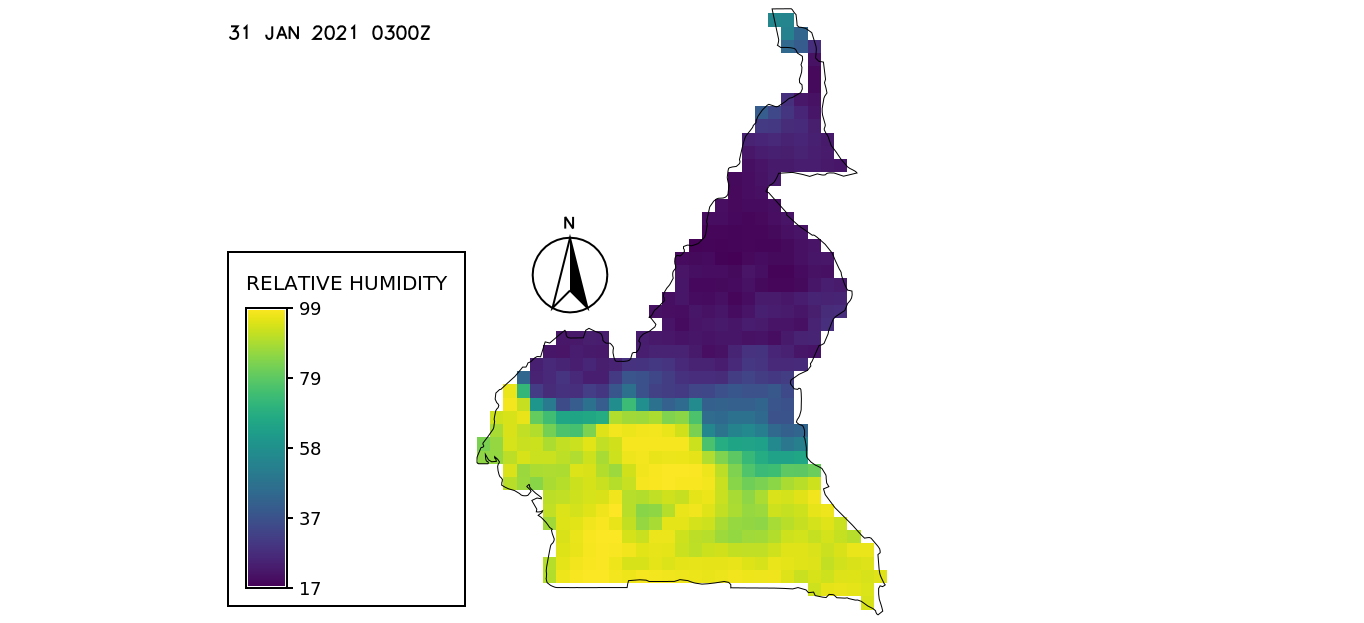
\includegraphics[scale=0.6]{rh03.png} %\cite{umhe}
\end{center}
\caption{Relative Humidity at 03:00 UTC}
\label{Relative Humidity at 03:00 UTC}%\cite{ABIA}
\end{figure}

\begin{figure}[H]
\begin{center}
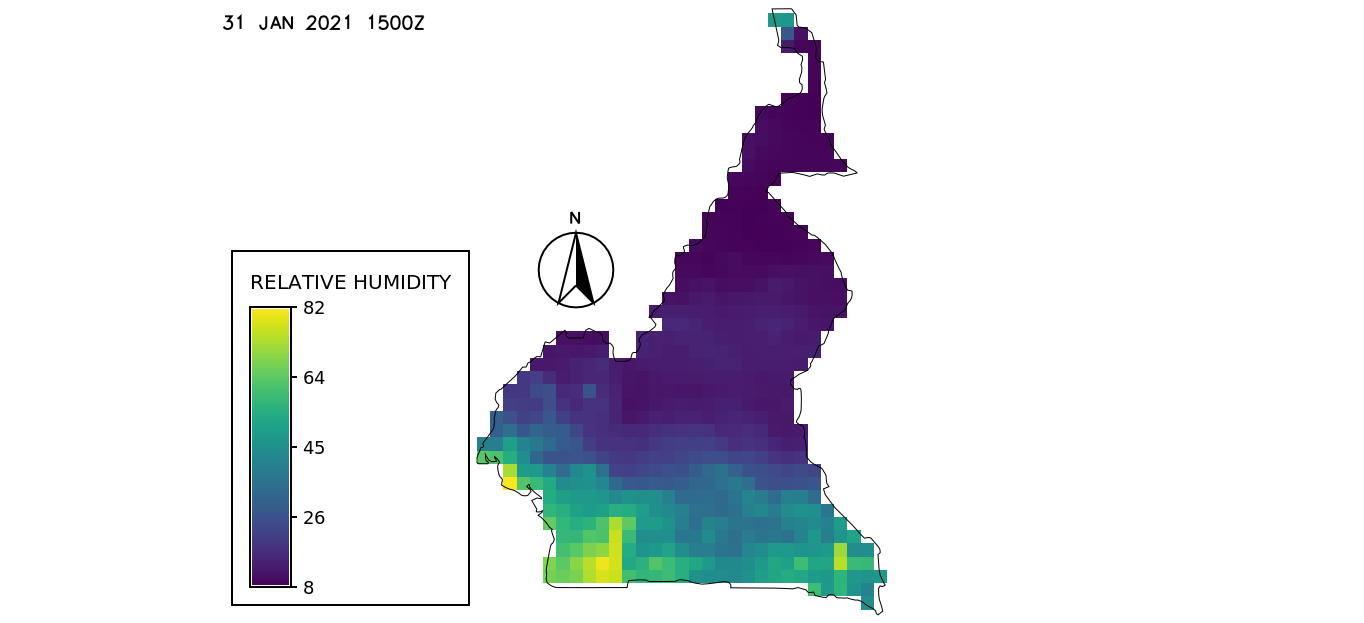
\includegraphics[scale=0.6]{rh15.png} %\cite{umhe}
\end{center}
\caption{Relative Humidity at 15:00 UTC}
\label{Relative Humidity at 15:00 UTC}%\cite{ABIA}
\end{figure}

\subsection{Surface Pressure Chart}
\begin{lstlisting}[language=Bash]
#dt="20210131.0300"
dt="20210131.1500"
# Visualize data
r.mask vect=cmr --o
# Open a monitor
d.mon wx0
# Display a raster map
d.rast GLDAS_NOAH025_3H_A${dt}_Psurf_final 
# Display a vector map
d.vect map=cmr type=boundary
d.text text="31 JAN 2021 1500Z" color=black bgcolor=white size=3
# Add raster legend
d.legend -t -s -b raster=GLDAS_NOAH025_3H_A${dt}_Psurf_final title="SURFACE PRESSURE (Pa)" title_fontsize=20 font=sans fontsize=18
# Add North arrow
d.northarrow style=1b text_color=black
#d.erase -f
#r.mask -r
\end{lstlisting}

\begin{figure}[H]
\begin{center}
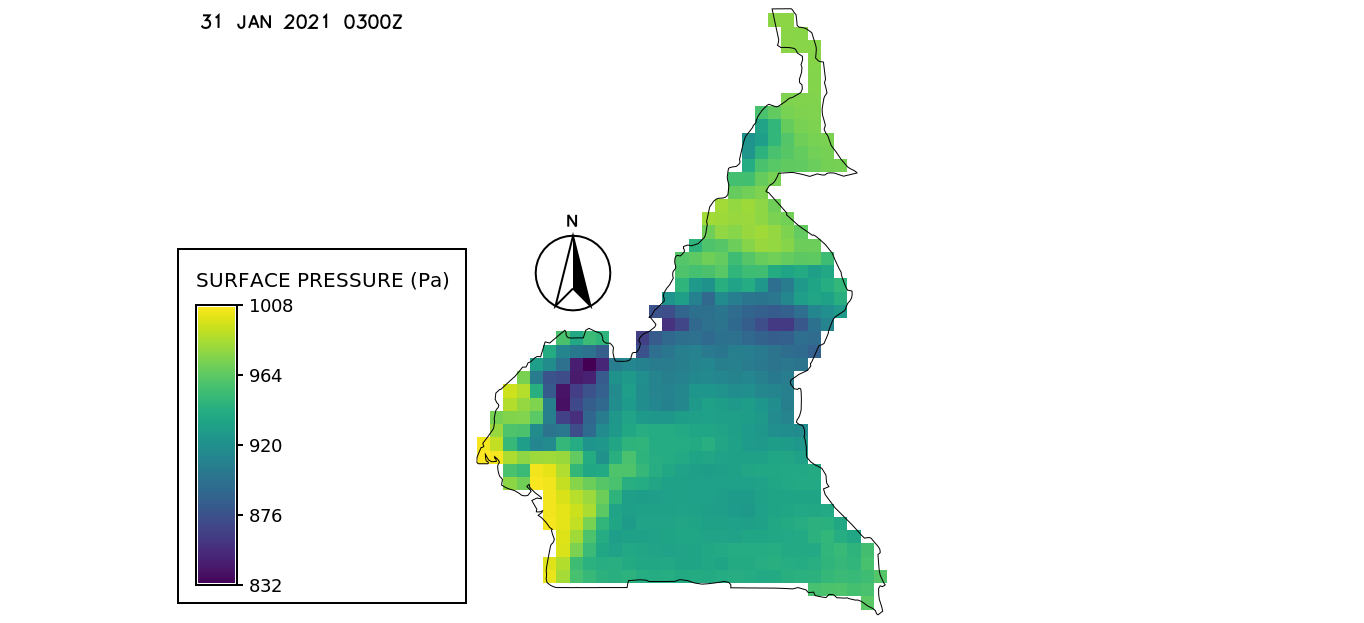
\includegraphics[scale=0.6]{sp03.png} %\cite{umhe}
\end{center}
\caption{Surface Pressure at 03:00 UTC}
\label{Surface Pressure  at 03:00 UTC}%\cite{ABIA}
\end{figure}

\begin{figure}[H]
\begin{center}
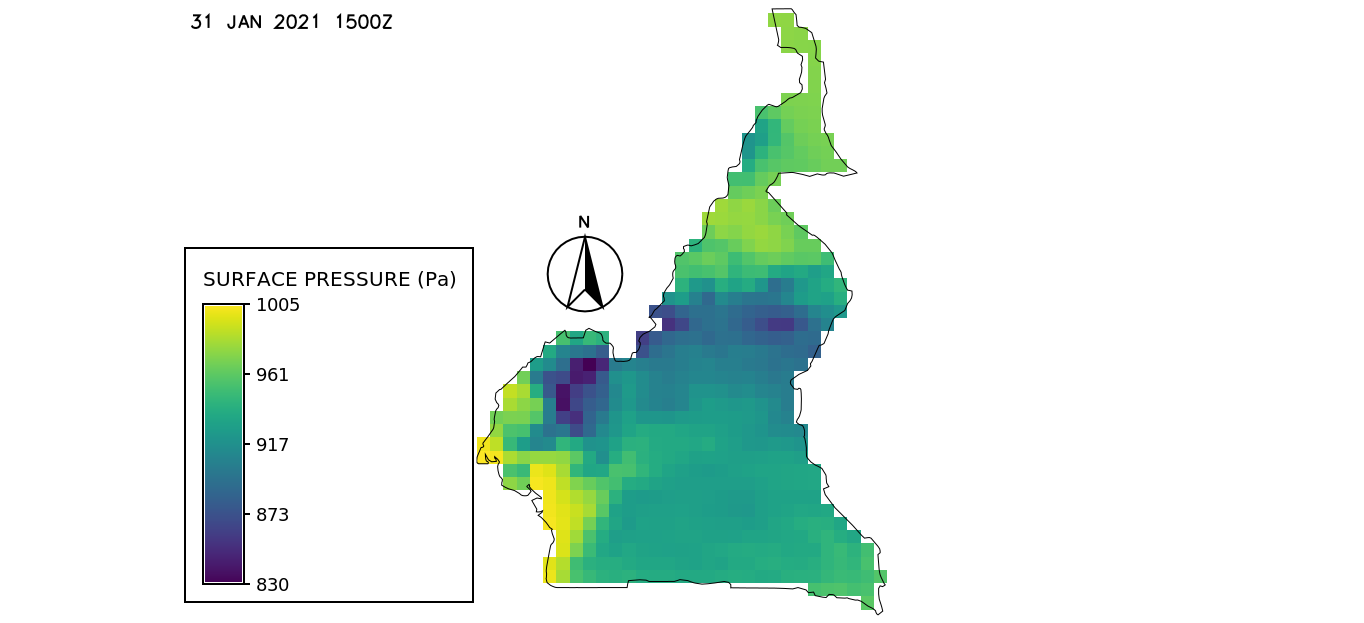
\includegraphics[scale=0.6]{sp15.png} %\cite{umhe}
\end{center}
\caption{Surface Pressure  at 15:00 UTC}
\label{Surface Pressure  at 15:00 UTC}%\cite{ABIA}
\end{figure}


\subsection{Wind Speed Chart}
\begin{lstlisting}[language=Bash]
#dt="20210131.0300"
dt="20210131.1500"
# Visualize data
r.mask vect=cmr --o
# Open a monitor
d.mon wx0
# Display a raster map
d.rast GLDAS_NOAH025_3H_A${dt}_Wind_final
# Display a vector map
d.vect map=cmr type=boundary
d.text text="31 JAN 2021 1500Z" color=black bgcolor=white size=3
# Add raster legend
d.legend -t -s -b raster=GLDAS_NOAH025_3H_A${dt}_Wind_final title="WIND SPEED m/s" title_fontsize=20 font=sans fontsize=18
#Add North arrowd.northarrow style=1b text_color=black
d.northarrow style=1b text_color=black
#d.erase -f
#r.mask -r

\end{lstlisting}

\begin{figure}[H]
\begin{center}
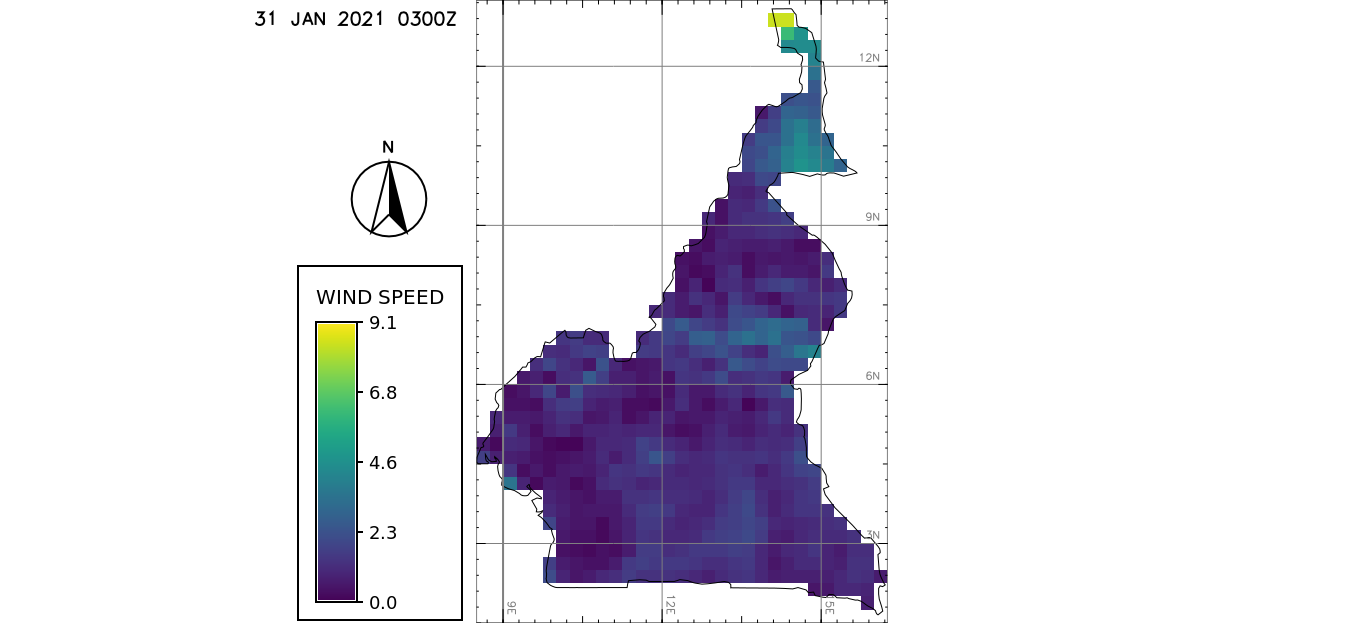
\includegraphics[scale=0.6]{ws03.png} %\cite{umhe}
\end{center}
\caption{Wind Speed at 03:00 UTC}
\label{Surface Pressure  at 03:00 UTC}%\cite{ABIA}
\end{figure}

\begin{figure}[H]
\begin{center}
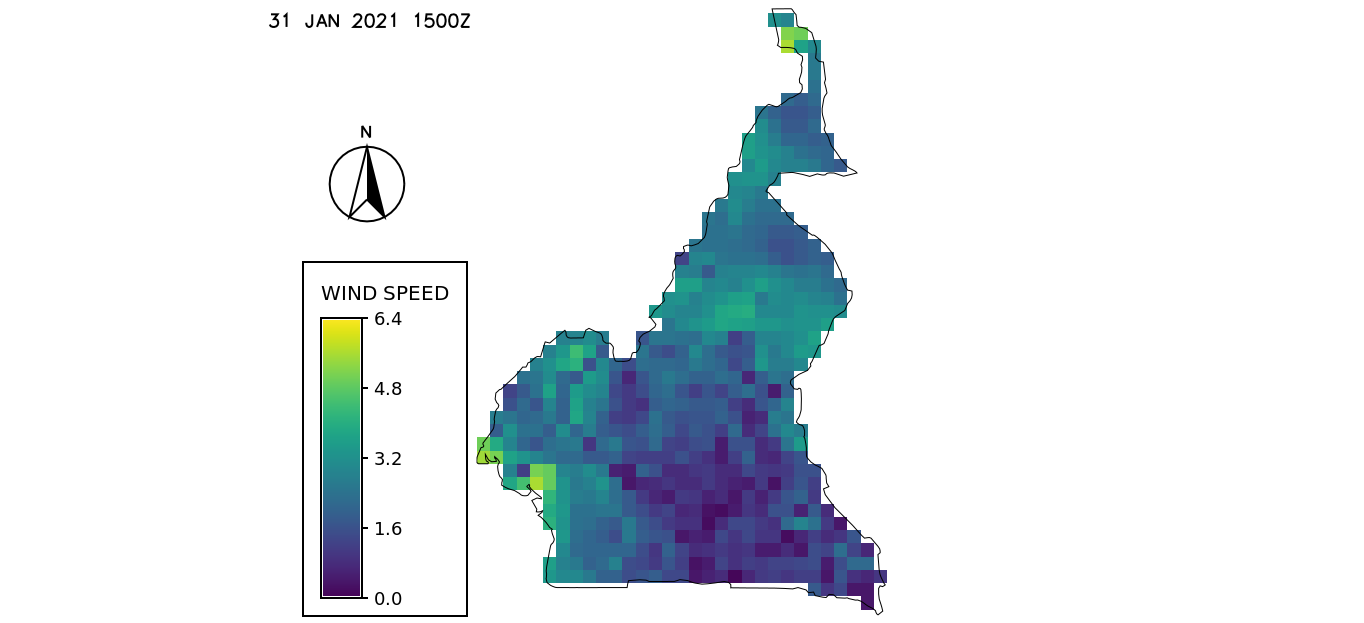
\includegraphics[scale=0.6]{ws15.png} %\cite{umhe}
\end{center}
\caption{Wind Speed at 15:00 UTC}
\label{Surface Pressure  at 15:00 UTC}%\cite{ABIA}
\end{figure}





\newpage

\chapter*{\normalsize{\textbf{CONCLUSION AND ADVANCEMENT}}}
%\addstarredchapter{CONCLUSION}
\addcontentsline{toc}{section}{\normalsize{\textbf{CONCLUSION AND ADVANCEMENT}}}
Meteorological satellite has proved to be very useful in weather analysis and forecasting.
Some of its applications are: 
\begin{itemize} 
\item Satellite imageries are used by the forecasters as first-hand information along with synoptic chart analysis while issuing the forecast.
\item Atmospheric sounding, clouds precipitation, convergence and divergence in the atmosphere, thunderstorm formation, various convective activities, can be derived / forecasted with the help of satellite pictures and their analysis. 
\item Cyclone formation, its intensity and movement (Track) can be monitored and predicted.
\end{itemize}
The advantages of meteorolgical satellite over ground observations  are :
\begin{itemize} 
\item Provides data of large region of the globe
\item Provides data of remote and inaccessible areas
\item Temporal data consistency 
\item Easy and rapid data collection
\item Relatively inexpensive
\item Rapid data interpretation
\end{itemize}
We also note some limitations of meteorolgical satellite as outlined below :
\begin{itemize} 
    \item Needs certain skill to interpret data
    \item Requires verification with ground observations
    \item Data from multiple sources may create confusion
    \item Objects can be misclassified
    \item Relative motion of sensor \& source may create 
    \item distortions in an image
\end{itemize}

\newpage

\end{document}
 